\setcounter{part}{27}  % s

\part{Signaux et électronique}
\section{\'Electronique en régime stationnaire}
% Niveau :      PCSI - PC
% Discipline :  Elec
% Mots clés :   Elec, Ordre 2

\begin{exercise}{Brèves}{1}{Sup,Spé}
{\'Electrocinétique, Circuits d'ordre 2}{bermu}

\begin{questions}
    \question Trois lampes à incandescence de puissances différentes (par exemple 25 W , 60 W et 100 W) sont reliées en
série ; l'ensemble est branché sur un générateur délivrant une tension de 220 V. \\
En admettant que
l'éclairement d'une lampe est proportionnel à la puissance électrique qu'elle reçoit, quelle lampe brillera le
plus fort ? Quid si les lampes sont en dérivation ? \\
N.B. : Ce qu'on appelle la puissance d'une lampe est sa puissance lorsqu'elle est soumise à une tension
caractéristique soit ici 220 V.

    \question Un poste de distribution EDF assimilé à une fem $E$ constante est relié à une installation domestique par deux
fils très longs dont la résistance totale inévitable est $r$. On appelle $P_f$ la puissance fournie par le poste de
distribution, $P_u$ la puissance utile reçue par l'installation et $\rho$ le rendement de l'opération. \\
Exprimer $\rho$ en fonction de $E$, $r$ et $P_f$ . En déduire que, pour une puissance fiéee, le rendement est d'autant
meilleur que $E$ est grand. Quelle est l'application pratique de ce résultat ?
\end{questions}
\end{exercise}
\begin{exercise}{Calculs d'impédance}{1}{Sup}
{\'Electrocinétique}{lelay}

\begin{questions}
    \questioncours Loi de composition des impédances et des admittances
    \question Quelle est l'impédance équivalente du circuit suivant ?
\begin{circuit}
      \draw
      (0,0) to [R, l^=$R$] (2,0) 
            to [L, l^=$C$] (4,0)
            to [C, l^=$C$] (6,0);
\end{circuit}
    \question Donner, pour chacun des circuits suivants, le rapport $s/e$
\end{questions}

\begin{circuit}
      \draw
      (0,0) to [open, v_=$e$, *-o] (0,2)
      (0,2) to [R, l=$R$] (2,2) 
      to [C, l^=$C$, *-*] (2,0)
      (2,2) to [short] (4,2)
      (4,0) to [open, v_=$s$, *-o] (4,2)
      (0,0) to [short] (4,0);
\end{circuit}

\begin{circuit}
      \draw
      (0,0) to [open, v_=$e$, *-o] (0,2)
      (0,2) to [R, l=$R$] (2,2) 
      to [C, l^=$C$, *-*] (2,0)
      (2,2) to [R, l=$R$] (4,2)
      to [C, l^=$C$, *-*] (4,0)
      (4,2) to [short] (6,2)
      (6,0) to [open, v_=$s$, *-o] (6,2)
      (0,0) to [short] (6,0);
\end{circuit}

\begin{circuit}
      \draw
      (0,0) to [open, v_=$e$, *-o] (0,2)
      (0,2) to [R, l=$R$] (2,2) 
      to [C, l^=$C$, *-*] (2,0)
      (2,2) to [R, l=$R$] (4,2)
      to [C, l^=$C$, *-*] (4,0)
      (4,2) to [R, l=$R$] (6,2)
      to [C, l^=$C$, *-*] (6,0)
      (6,2) to [short] (8,2)
      (8,0) to [open, v_=$s$, *-o] (8,2)
      (0,0) to [short] (8,0);
\end{circuit}

\end{exercise}

\begin{solution}

avec $p = jRC\omega = j\frac{\omega}{\omega_0}$
\begin{align*}
    \frac{s}{e} &= \frac{1}{1+p} \\
    \frac{s}{e} &= \frac{1}{(1+p)(2+p)-1} \\
    \frac{s}{e} &= \frac{1}{(1+p)(2+p)^2-1} \\
\end{align*}
\end{solution}
% Niveau :      PCSI - PC
% Discipline :  Elec
% Mots clés :   Elec, Ordre 2

\begin{exercise}{Résistance d'un maillage}{2}{Sup,Spé}
{\'Electrocinétique, Circuits d'ordre 2}{schlosser}

On s'intéresse à la résistance d'un maillage pris entre deux points.

\begin{questions}
    \questioncours Dipôles actifs et passifs : caractéristique, résistance et conductance. Association de dipôles.
    \question Quelle est la résistance d'une maille simple (Circuit \arabic{exercise}.1) ?
    \question Quelle est la résistance d'une maille double (Circuit \arabic{exercise}.2) ?
\begin{EnvUplevel}
    Dans les figures ci-dessous, toutes les résistances valent $R$.
\begin{multicols}{2}
\begin{circuit}[Maille simple]
    \draw (0,0)
    to [R] (2,0)
    to [R] (2,2)
    to [R] (0,2)
    to [R] (0,0) ;
    \draw (-.4,2.4) to [short, *-*] (0,2);
    \draw (2,0) to [short, *-*] (2.4,-.4);
\end{circuit}
\begin{circuit}[Maille double]
    \draw (0,0)
    to [R] (2,0)
    to [R] (4,0)
    to [R] (4,2)
    to [R] (4,4)
    to [R] (2,4)
    to [R] (0,4)
    to [R] (0,2)
    to [R] (0,0);
    \draw (2,4)
    to [R, *-*] (2,2)
    to [R, *-*] (2,0) ;
    \draw (4,2)
    to [R, *-*] (2,2)
    to [R, *-*] (0,2) ;
    \draw (-.4,4.4) to [short, *-*] (0,4);
    \draw (4,0) to [short, *-*] (4.4,-.4);
\end{circuit}
\end{multicols}

Et maintenant l'astuce !
\end{EnvUplevel}
    \question Monter que les courts-circuits coupant perpendiculairement les axes de symétrie et d'antisymétrie de la répartition des courants peuvent être supprimés sans modifier la répartition des courants.
    
    \question Retrouver par cette  méthode le résultat de la question 3.
    
    \question Donner le résultat pour la maille triple :
\end{questions}
    
\begin{circuit}[Maille triple]
    \draw (0,0)
    to [R] (2,0)
    to [R] (4,0)
    to [R] (6,0)
    to [R] (6,2)
    to [R] (6,4)
    to [R] (6,6)
    to [R] (4,6)
    to [R] (2,6)
    to [R] (0,6)
    to [R] (0,4)
    to [R] (0,2)
    to [R] (0,0);
    \draw (2,0)
    to [R, *-*] (2,2)
    to [R, *-*] (2,4)
    to [R, *-*] (2,6) ;
    \draw (4,0)
    to [R, *-*] (4,2)
    to [R, *-*] (4,4)
    to [R, *-*] (4,6) ;
    \draw (0,2)
    to [R, *-*] (2,2)
    to [R, *-*] (4,2)
    to [R, *-*] (6,2) ;
    \draw (0,4)
    to [R, *-*] (2,4)
    to [R, *-*] (4,4)
    to [R, *-*] (6,4) ;
    \draw (-.4,6.4) to [short, *-*] (0,6);
    \draw (6,0) to [short, *-*] (6.4,-.4);
\end{circuit}

C'est plus rapide comme ça, non ?

%\plusloin Quid du cas de la $n$-maille ?

\end{exercise}

\begin{solution}
    \url{https://fr.wikiversity.org/wiki/Signaux\_physiques\_(PCSI)/Exercices/Circuits\_\%C3\%A9lectriques\_dans\_l\%27ARQS\_:\_associations\_de\_conducteurs\_ohmiques}
\end{solution}

\section{\'Electronique en régime transitoire}
% Niveau :      PCSI - PC
% Discipline :  Elec
% Mots clés :   Elec, Ordre 2

\begin{exercise}{Tube fluorescent}{1}{Sup,Spé}
{\'Electrocinétique, Circuits d'ordre 2}{bermu}


Les tubes fluorescents sont un type particulier de lampes électriques qui produisent de la lumière grâce à une décharge électrique.

Ces tubes s'allument quand la tension à leur bornes dépasse une certaine tension d'allumage $U_a$. Un fois allumé, le tube s'éteint quand la tension descend en dessous de $U_e$, la tension d'extinction, comme l'illustre la figure ci-dessous.

\begin{figure}[H]
    \centering
    \includegraphics[width=0.65\linewidth]{elec/neon.jpg}
    \caption{Tension au bornes du néon $u_\textsc{c}$ en fonction du temps.}
\end{figure}

\`A $t<0$, le condensateur $C$ est déchargé et le tube est éteint. On allume le générateur à $t=0$.

Le circuit électrique, dans lequel est inséré le tube fluorescent, est schématisé ci-dessous :
\begin{circuit}[Modélisation du tube néon.]
      \draw (0,0)
      to [vsource, v^>=$E$] (0,3)
      to [R, l=$R$] (2,3)
      to [C, l_=$C$, *-*] (2,0)
      to [short] (0,0) {}
      (2,3) to [short] (4,3)
      to [nos, l^=$K$] (4,2)
      to [R, l^=$r$] (4,0)
      to [short] (2,0) {}
      (2.7,0) [open, v_=$u_\textsc{c}$] to (2.7,3) {} ;
      \draw [red, dashed] (3.6,-0.2) rectangle(4.8,3.2) ;
      \node [red] at (4.2,3.5) {Tube néon};
\end{circuit}
Le tube fluorescent est modélisé comme une résistance faible $r$ et un interrupteur $K$ en série. L'interrupteur est ouvert lorsque le tube est éteint et fermé lorsque le tube est allumé.
% Le tube fluorescent est modélisé comme une résistance faible $r$ et un interrupteur $K$ qui s'ouvre et se ferme selon si le tube est allumé ou éteint.

\paragraph{Données :} $E = 100$ V, $R = 60$ k$\Omega$, $r = 10$ $\Omega$, $C = 600$ nF.


\begin{questions}
    \questioncours Condensateurs et dipôles à comportement capacitifs.
    
    \question Décrire le comportement global observé en Fig.~\arabic{exercise}.1 ci-dessus et donner les valeurs de $U_e$ et $U_a$.
    
    \uplevel{On étudie d'abord le circuit entre $t = 0$ et $t_1$.}
    
    \question Simplifier le circuit \arabic{exercise}.1 dans ce cas puis résoudre l'équation différentielle vérifiée par $i$ et $u_\textsc{c}$.
    \question Calculer le temps $t_1$ de l'allumage du néon. Par analogie, quel est le temps $\tau$ du cycle d'allumage du néon ?
    
    \uplevel{On étudie maintenant d'abord le circuit entre $t_1$ et $t_1 + \varepsilon$.}
     
    \question En remarquant que $R\gg r$, simplifier le circuit \arabic{exercise}.1 dans ce cas puis résoudre l'équation différentielle vérifiée par $i$ et $u_\textsc{c}$.
    \question Calculer le temps $t'$ de décharge du condensateur. Justifier que l'on peut négliger ce temps dans le cycle du néon. Voit-on le néon s'allumer et s'éteindre ?
    
\end{questions}
\end{exercise}
% Niveau :      PCSI
% Discipline :  Elec
% Mots clés :   Elec, Ordre 1

\begin{exercise}{Combinaison de dipôles}{1}{Sup}
{\'Electrocinétique, Circuits d'ordre 1}{lelay,mines}

On cherche à décrire le circuit suivant :
\begin{circuit}
      \draw
      node [ground] at (0,0) {}
      to [vsource, v^>=$E$, i^>=$i$] (0,2)
      to [short] (1,2)
      
      (1,2) to [short] (1,1)
      to [short] (2,1)
      to [R, l^=$R_2$] (3,1)
      to [short] (4,1)
      to [short] (4,2)
      
      (1,2) to [short] (1,3)
      to [short] (2,3)
      to [R, l^=$R_1$] (3,3)
      to [short] (4,3)
      to [short] (4,2)
      
      (4,2) to [short] (5,2)
      to [R, l^=$R_0$] (6,2)
      to [short] (7,2)
      
      (7,2) to [short] (8,2)
      
      (8,2) to [short] (8,1)
      to [short] (9,1)
      to [L, l^=$L_2$] (10,1)
      to [short] (11,1)
      to [short] (11,2)
      
      (8,2) to [short] (8,3)
      to [short] (9,3)
      to [L, l^=$L_1$] (10,3)
      to [short] (11,3)
      to [short] (11,2)
      
      (11,2) to [short] (12,2)
      to [L, l^=$L_0$] (13,2)
      to [short] (14,2)
      
      to [short] (14,0)
      node [ground]{};
\end{circuit}

\begin{questions}
    \questioncours Loi de composition des résistances en série et en parallèle. (Si vous l'avez vu : ) Pont diviseur de tension.
    \question Écrire l'équation régissant le courant $i$ passant  dans le circuit plus haut et montrez que cette équation peut se mettre sous la forme
    \begin{align*}
        L \dv{i}{t} + Ri = E
    \end{align*}
    Où $L$ (resp. $R$) est une inductance (resp. résistance) fonction de $L_0$, $L_1$ et $L_2$ (resp. $R_0$, $R_1$, $R_2$) que l'on précisera.
    \question La forme revêtue par $L$ vous semble-t-elle familière ? Justifier que les bobines se comportent `un peu comme' des résistances.
    \question Écrire maintenant l'équation régissant l'évolution de la tension $u$ dans le circuit suivant et montrez que cette équation peut se mettre sous la forme
    \begin{align*}
        C \dv{u}{t} + \frac{u}{R} = I
    \end{align*}
    Où $C$ (resp. $R$) est une capacité (resp. résistance) fonction de $C_0$, $C_1$ et $C_2$ (resp. $R_0$, $R_1$, $R_2$) que l'on précisera.
    
\begin{circuit}
      \draw
      node [ground] at (0,0) {}
      to [short] (0,2)
      to [short] (1,2)
      
      (1,2) to [short] (1,1)
      to [short] (2,1)
      to [R, l^=$R_2$] (3,1)
      to [short] (4,1)
      to [short] (4,2)
      
      (1,2) to [short] (1,3)
      to [short] (2,3)
      to [R, l^=$R_1$] (3,3)
      to [short] (4,3)
      to [short] (4,2)
      
      (4,2) to [short] (5,2)
      to [R, l^=$R_0$] (6,2)
      to [short] (7,2)
      
      node [ground] at (7,0) {}
      (7,0) to [isource, v^>=$u$, i^>=$I$] (7,2)
      
      (7,2) to [short] (8,2)
      
      (8,2) to [short] (8,1)
      to [short] (9,1)
      to [C, l^=$C_2$] (10,1)
      to [short] (11,1)
      to [short] (11,2)
      
      (8,2) to [short] (8,3)
      to [short] (9,3)
      to [C, l^=$C_1$] (10,3)
      to [short] (11,3)
      to [short] (11,2)
      
      (11,2) to [short] (12,2)
      to [C, l^=$C_0$] (13,2)
      to [short] (14,2)
      
      to [short] (14,0)
      node [ground]{};
\end{circuit}

    \question Proposer une loi de composition en série et en parallèle des bobines et des condensateurs.
\end{questions}
\end{exercise}


\begin{solution}

\begin{questions}
    \questioncours ok
    \question $E$
    \question $t = 0$, la bobine est un interrupteur ouvert, $t=\infty$, le condensateur est un fil
    \question $3L \dv{u}{t} + R u = 0$
    \question $\tau = 3L/R$
    \question Une exponentielle décroissante pépère.
\end{questions}

\end{solution}
% Niveau :      PCSI
% Discipline :  Elec
% Mots clés :   Elec, Ordre 1

\begin{exercise}{Bobine avec interrupteur}{1}{Sup}
{\'Electrocinétique, Circuits d'ordre 1}{lelay}

On cherche à décrire le circuit suivant :
\begin{circuit}
      \draw
      node [ground] at (0,0) {}
      to [vsource, v^>=$E$] (0,2)
      to [R, l^=$R$] (2,2)
      to [nos, l=$K$] (4,2)
      to [R, l^=$R$] (6,2)
      to [vsource, v^<=$E$] (6,0)
      node [ground]{}
      (2,2) to [R, l_=$R$] (2,0)
      node [ground]{}
      (4,2) to [L, l^=$L$] (4,0)
      node [ground]{};
\end{circuit}

\begin{questions}
    \questioncours Donne la loi reliant la tension aux bornes d'une bobine au courant qui la traverse. Unité et ordre de grandeur de l'inductance d'une bobine.
    \question Quelle est la tension aux bornes de la bobine tant que l'interrupteur reste ouvert ? Le courant qui la traverse ?
    \question À $t = 0$, on ferme l'interrupteur $K$. Donner le circuit équivalent à $t = 0^+$ et à $t = \infty$.
    \question Donner l'équation différentielle vérifiée par la tension $u$ aux bornes de la bobine.
    \question Quel est le temps caractéristique d'évolution de $u(t)$ ? Quel nom proposez-vous de lui donner ?
    \question Écrire $u(t)$ et donner l'allure de sa courbe.
\end{questions}
\end{exercise}


\begin{solution}

\begin{questions}
    \questioncours ok
    \question $E$
    \question $t = 0$, la bobine est un interrupteur ouvert, $t=\infty$, le condensateur est un fil
    \question $3L \dv{u}{t} + R u = 0$
    \question $\tau = 3L/R$
    \question Une exponentielle décroissante pépère.
\end{questions}

\end{solution}
% Niveau :      PCSI
% Discipline :  Elec
% Mots clés :   Elec, Ordre 1

\begin{exercise}{Condensateur avec interrupteur}{1}{Sup}
{\'Electrocinétique, Circuits d'ordre 1}{lelay}

On cherche à décrire le circuit suivant :
\begin{circuit}
      \draw
      node [ground] at (0,0) {}
      to [vsource, v^>=$E$] (0,2)
      to [R, l^=$R$] (2,2)
      to [nos, l=$K$] (4,2)
      to [R, l^=$R$] (6,2)
      to [vsource, v^<=$E$] (6,0)
      node [ground]{}
      (2,2) to [R, l_=$R$] (2,0)
      node [ground]{}
      (4,2) to [C, l^=$C$] (4,0)
      node [ground]{};
\end{circuit}

\begin{questions}
    \questioncours Donne la loi reliant la tension aux bornes d'un condensateur à la charge qu'il contient. Unité et ordre de grandeur de la capacité d'un condensateur.
    \question Quelle est la tension aux bornes du condensateur tant que l'interrupteur reste ouvert ? Le courant qui le traverse ?
    \question À $t = 0$, on ferme l'interrupteur $K$. Donner le circuit équivalent à $t = 0^+$ et à $t = \infty$.
    \question Donner l'équation différentielle vérifiée par la tension $u$ aux bornes du condensateur.
    \question Quel est le temps caractéristique d'évolution de $u(t)$ ? Quel nom proposez-vous de lui donner ?
    \question Écrire $u(t)$ et donner l'allure de sa courbe.
\end{questions}
\end{exercise}


\begin{solution}

\begin{questions}
    \questioncours ok
    \question $E$
    \question $t = 0$, le condensateur est un fil, $t=\infty$, le condensateur est un interrupteur ouvert
    \question $RC \dv{u}{t} + 3 u = 2e$
    \question $\tau = RC/3$
    \question Une exponentielle saturante pépère.
\end{questions}

\end{solution}
% Niveau :      PCSI - PC
% Discipline :  Elec
% Mots clés :   Elec, Ordre 2

\begin{exercise}{Circuit avec interrupteur}{2}{Sup,Spé}
{\'Electrocinétique, Circuits d'ordre 2}{lelay,mines}

On cherche à décrire le circuit suivant :
\begin{circuit}
      \draw
      node [ground] at (0,0) {}
      to [short] (0,1)
      to [vsource, v^>=$E$] (0,3) 
      to [short] (0,4)
      to [nos, l=$K$] (2,4)
      to [C, l_=$C$, *-*] (2,2)
      to [R, l_=$R$] (2,0)
      node [ground]{}
      (2,4) to [short] (5,4)
      to [R, l^=$R$, -*] (5,2)
      to [C, l^=$C$] (5,0)
      node [ground]{}
      (2,2) to [short, i_=$i$] (3,2) 
      to [R, l^=$R$] (5,2);
\end{circuit}
Initialement, les condensateurs $C$ sont déchargés.

\begin{questions}
    \questioncours Donne la loi reliant la tension aux bornes d'un condensateur à la charge qu'il contient.
    \question On considère le circuit ci-dessus. À $t = 0$, on ferme l'interrupteur $K$. 
    \question Donner le circuit équivalent à $t = 0^+$ et à $t = \infty$.
    \question En déduire $i(t = 0^+)$ et $i(t = \infty)$. Justifier qu'il y a un instant $t_0$ pour lequel $i(t_0) = 0$.
    \question Donner l'équation différentielle vérifiée par $i$ et en déduire $i(t)$.
    \question Donner $t_0$.
\end{questions}
\end{exercise}


\begin{solution}


Par symétrie, la tension aux bornes des deux condensateurs est la même, notée $u$ (si pas convaincu: écrire le système et vérifier que $u_{C_1}-u_{C_2} = 0$).

Du coup (loi des mailles) : la tension aux bornes des deux résistances sur le coté est $u-E$.

On a donc (loi des mailles sur une maille intérieure) : $u + Ri + u-E = 0$ et (loi des noeuds sur un des noeuds) : $i = \frac{u-E}{R} + C\dv{u}{t}$. On en déduit immédiatement que $u = (E-Ri)/2$ et donc que $i$ satisfait $\dv{i}{t} + \frac{3i}{\tau} = \frac{-1}{\tau}\frac{E}{R}$, donc $i(t) = \frac{E}{R}-\frac{4}{3}\frac{E}{R}e^{3t/\tau}$ donc $t_0 = \frac{\tau}{3}\ln\qty(\frac43)$
\begin{circuit}
      \draw
      node [ground] at (0,0) {}
      to [short] (0,1)
      to [vsource, v^>=$E$] (0,3) 
      to [short] (0,4)
      to [short] (2,4)
      to [C, v_<=$u$] (2,2)
      to [R, v_>=$u - E$] (2,0)
      node [ground]{}
      (2,4) to [short] (5,4)
      to [R, v^>=$u - E$] (5,2)
      to [C, v^<=$u$] (5,0)
      node [ground]{}
      (2,2) to [R, v^<=$Ri$] (5,2);
\end{circuit}

\end{solution}
% Niveau :      PCSI
% Discipline :  Elec
% Mots clés :   Elec, Ordre 2

\begin{exercise}{Condensateurs couplés}{2}{Sup}{\'Electrocinétique, Circuits d'ordre 2}{correge}

On considère le schéma suivant. Les condensateurs de même capacité $C$ sont déchargés lorsque les interrupteurs $K_1$ et $K_2$ sont ouverts.

\begin{figure}[H]
\centering
\includegraphics[scale=0.9]{elec/CondCouples.pdf}
\end{figure}

\begin{questions}

    \question En régime continu, par quels éléments peut-on remplacer condensateurs et bobines ?
    \question On ferme $K_1$, $K_2$ restant ouvert. Déterminer en un minimum de calcul  les charges $q_1$ et $q_2$ portées par les deux condensateurs identiques au bout d'un temps très long.
    \question Quelle est alors l'énergie emmagasinée par le système ? \\
              Application numérique pour $C=1\mu$F et $E=10$V.
    \question À partir de maintenant, on ferme $K_2$, $K_1$ restant fermé, et on prend une nouvelle origine des temps.
              Que vaudront l'intensité $i_0$ dans la bobine et les charges $q_1$ et $q_2$ au bout d'un temps long ? \\
              Indication : commencer par dessiner un schéma équivalent au bout d'un temps très long, et raisonner sur ce schéma à l'aide des lois de Kirchhoff.
    \question Quelles sont l'intensité $i_0$ dans la bobine et les charges $q_1$ et $q_2$ des condensateurs à $t=0^+$ ? Justifier.
    \question Écrire les lois de Kirchhoff et les lois usuelles pour les divers composants, puis établir deux équations différentielles du second ordre que vérifient les charges $q_1$ et $q_2$ des deux condensateurs après la fermeture de $K_2$.
    \question On suppose à partir d'ici que $r=R$. Montrer qu'à partir des deux équations différentielles précédentes, on obtient une équation sur $Q=q_1+q_2$ et une équation sur $q=q_1-q_2$.
    \question Résoudre ces équations, donner l'expression de $Q(t)$ et $q(t)$, et montrer en particulier que $Q$ est effectivement indépendante du temps.
    \question Les autres valeurs des composants sont prises à $L_0=5$mH, $r=200\Omega$. \\
              Montrer que 
              \[i_0(t) = \frac{r^2 C E}{16 L_0^2} t\cdot\exp\left(-\frac{r}{4L_0}t\right),\]
              et représenter graphiquement l'allure de $i_0(t)$.
\end{questions}



\end{exercise}

\begin{solution}
\begin{questions}
    \question En régime continu, une bobine est équivalente à un fil, alors qu'un condensateur est équivalent à un interrupteur ouvert.
    \question  Au bout d'un temps long, les condensateurs se comportent comme des coupe-circuits. Le courant circulant dans le circuit est donc nul. Par suite, la loi des mailles donne
                \begin{equation}
                E = u_1+u_2
                \end{equation}
                avec $u_1$ et $u_2$ les tensions aux bornes des condensateurs. Mais comme les deux condensateurs sont reliés par un fil, en régime permanent, la charge portée par leurs armatures est nécessairement la même. D'où $q_1=q_2=q$, et par suite 
                \begin{equation}
                E=2\times\frac{q}{C} \quad \Longrightarrow \quad \boxed{q = \frac{CE}{2}}
                \end{equation}
    \question On a alors l'énergie $W$ emmagasinée par le système
                \begin{equation}
                W = 2\times\frac{1}{2}\frac{q^2}{C} = \frac{CE^2}{4} = 2,5.10^{-5}J
                \end{equation}
    \question Pour un temps long, la bobine est équivalente à un fil. On a toujours $i_1=i_2=0$ car les condensateurs bloquent le courant, et par la loi des noeuds $i_0=0$. 
              En appliquant la loi des mailles dans la maille de gauche, on a $u_1=E$ (pas de tension aux bornes des résistances), donc $q_1=CE$. Dans la maille de droite, $u_2=0$ donc $q_2=0$.
    \question Par continuité de l'intensité traversant une bobine, $i_0(0^+)=0$. Par ailleurs, la charge au borne d'un condensateur est une fonction continue (car la tension l'est), donc on a $q_1(0^+)=q_2(0^+)=\frac{CE}{2}$.
    \question On écrit la loi des mailles dans les mailles de droite et de gauche :
                \begin{align}
                    E &= u_0+u_1+Ri_1 \\
                    0 &= u_0-u_2-ri_2
                \end{align}
                On a bien sûr $i_1=i_0+i_2$. 
                Par ailleurs, $u_1 = \frac{q_1}{C}, u_2=\frac{q_2}{C}$, et finalement:
                \begin{equation}
                    u_0=L_0\dv{i_0}{t}=L_0\dv{(i_1-i_2)}{t} = L_0\left(\dv{ q_1}{t}-\dv{q_2}{t}\right).
                \end{equation}
                En réarrangeant les équations de mailles, on obtient donc les équations différentielles couplées

                \begin{equation}
                \label{eqcouple}
                \boxed{
                \left\{\begin{array}{ll}
                \dv{ q_1}{t}-\dv{ q_2}{t}+\frac{R}{L_0}\dv{q_1}{t}+\frac{q_1}{L_0 C} = \frac{E}{L_0}\\
                \dv{q_1}{t}-\dv{ q_2}{t}-\frac{r}{L_0}\dv{q_2}{t}-\frac{q_2}{L_0 C} = 0 \\
                \end{array}\right.}
                \end{equation}
    \question  Les équations présentées ici sont caractéristiques de ce qu'on appelle des modes symétriques et antisymétriques (vous les retrouverez en TP lors de l'étude des pendules couplés). L'astuce habituelle pour les découpler consiste à faire apparaître les combinaisons $Q=q_1+q_2$ et $q=q_1-q_2$. Puis, prenant (\ref{eqcouple}), et calculant la somme et la différence des deux équations, on obtient finalement

                \begin{equation}
                \boxed{ \left\{\begin{array}{ll}
                    \dv{q}{t}+\frac{r}{2L_0}\dv{q}{t}+\frac{q}{2L_0 C} = \frac{E}{2L_0} \\
                    \dv{Q}{t}+\frac{Q}{rC} = \frac{E}{r} 
                \end{array}\right.}
                \end{equation}
    \question Résolvons l'équation différentielle pour $Q$. Il s'agit d'une équation différentielle du premier ordre avec second membre. La solution de l'équation homogène associée est $Q_H(t) = Ke^{-t/rC}$. Une solution particulière est $Q_p(t) = CE$. La condition initiale est 

                \begin{equation}
                Q(0) = q_1(0)+q_2(0) = CE \Rightarrow K+CE = CE \Rightarrow K=0 !
                \end{equation}

                Ainsi, $\boxed{Q(t)=CE=\text{cste}}$ : la charge totale des deux condensateurs reste constante.

                On résout maintenant l'équation différentielle associée à $q$. Il s'agit d'une équation du second ordre. On commence par résoudre l'équation sans second membre. L'équation caractéristique est
                \[x^2+\frac{r}{2L_0}x+\frac{1}{2L_0C}=0.\]

                Son discriminant vaut $\Delta = \frac{r^2}{4L_0^2}-\frac{2}{L_0C} \approx 0$ avec le degré de précision des données du problème. On a donc une racine double $x=\frac{r}{4L_0}$, et la solution se met sous la forme $q_H(t) = (At+B)\exp\left(-\frac{r}{4L_0}t\right)$. Une solution particulière étant $q_p(t)=CE$, on a alors 

                \begin{equation}
                q(t) = CE+(At+B)\exp\left(-\frac{r}{4L_0}t\right).
                \end{equation}

                Les conditions initiales sont $q(0^+) = q_1(0^+)-q_2(0^+) = 0$, ce qui amène $B=-CE$. Par ailleurs, $\dv{q}{t}(0^+) = \dv{q_1}{t}(0^+)-\dv{q_2}{t}(0^+) = i_1(0^+)-i_2(0^+) = i_0(0^+) = 0$, et $\dv{q}{t} = (A-\frac{r}{4L_0}(At-CE))\exp\left(-\frac{r}{4L_0}t\right) = A+\frac{rCE}{4L_0}$, soit $A=-\frac{rCE}{4L_0}$. Finalement 

                \begin{equation}
                q(t) = CE\left(1-(1+\frac{r}{4L_0}t)e^{-\frac{r}{4L_0}t}\right).
                \end{equation}
    \question On sait que $i_0 = i_1-i_2$, donc $i_0=\dv{q}{t}$, ce qui donne
                \begin{equation}
                    i_0(t)=CE\left(-\frac{r}{4L_0}+\frac{r}{4L_0}(1+\frac{r}{4L_0})\right)\exp(-\frac{r}{4L_0}t)
                \end{equation}
                \begin{equation}
                \boxed{i_0(t) =\frac{r^2CE}{16L_0^2}t.\exp\left(-\frac{r}{4L_0}t\right)}
                \end{equation}
\end{questions}

\end{solution}
% Niveau :      PCSI
% Discipline :  Elec
% Mots clés :   Elec, Ordre 2

\begin{exercise}{Décrement logarithmique}{2}{Sup}{\'Electrocinétique, Circuits d'ordre 2}{correge}

Dans le montage ci-dessous, le générateur de tension est idéal, de force électromotrice $E$ constante. Tant que l'interrupteur est ouvert, le condensateur est déchargé et la bobine (idéale) n'est parcourue par aucun courant. À l'instant $t=0$, on ferme l'interrupteur.

\begin{figure}[H]
\centering
\includegraphics[scale=1]{elec/circuitDecrement.pdf}
\end{figure}

\begin{questions}
    \question Déterminer par raisonnements simples la tension $u$ et les courants $i_R, i_L,i_C$ et $i$ (dans l'ordre qui vous paraîtra le plus judicieux):  à $t=0^-$, à $t=0^+$ et à $t\to \infty$.
    
    \question Établir l'équation différentielle régissant l'évolution de $i_R$ (on pourra écrire la loi des noeuds et la dériver). On posera pour ce circuit parallèle :
              \[\omega_0 = \frac{1}{\sqrt{LC}} \qquad \lambda = \frac{R+r}{2rRC}\]
    \question Pour la suite, on prendra $R=\SI{2,50}{k\ohm}, r=\SI{1,25}{k\ohm}, C=\SI{1,00}{\micro\farad}, L=\SI{20,0}{mH}, E=\SI{6,00}{V}$. À quel type de régime transitoire assiste-t-on ? Justifier.
    \question Définir et calculer la pseudo-pulsation $\omega$ et la pseudo-période $T$ du phénomène. Compte-tenu de la précision des données, que peut-on dire des valeurs numériques comparées de $\omega$ et $\omega_0$ ?
    \question Écrire la solution de l'équation différentielle en $i_R$ obtenue à la question 2 et satisfaisant aux conditions initiales trouvées à la question 1.
    \question En déduire alors l'expression de $u(t)$ et tracer l'allure du graphe correspondant. Donner l'instant $t_0$ auquel $u$ atteint sa valeur maximale.
    \question On définit le décrément logarithmique de $u$ par 
              \[\delta = \frac{1}{n}\ln\left(\frac{u(t)}{u(t+nT)}\right)\]
              Exprimer $\delta$ en fonction de $\lambda$ et $T$. Application numérique.
\end{questions}
\end{exercise}

%vides ?
%\input{elec/ALI}
%\input{elec/autourdurlc}


\section{\'Electronique en régime sinusoïdal forcé}
\begin{exercise}{Quelques (pré) filtres (1)}{1}{Sup}
{\'Electrocinétique}{lelay}

\begin{questions}
    \questioncours Notion de déphasage, d'avance et de retard de phase
    \question Donner le déphasage entre $\underline{s}$ et $\underline{e}$ dans le circuit suivant en fonction de la fréquence $\omega$ de $\underline{e}$
\begin{circuit}
      \draw
      (0,0) to [open, v_=$\underline{e}$, *-o] (0,2)
      (0,2) to [R, l=$R$] (2,2) 
      to [C, l^=$C$, *-*] (2,0)
      (2,2) to [short] (4,2)
      (4,0) to [open, v_=$\underline{s}$, *-o] (4,2)
      (0,0) to [short] (4,0);
\end{circuit}
    \question Pour quelle valeur de $\omega$ a-t-on un déphasage de $-\pi/3$ ?
    \question Tracer la courbe $\Delta\varphi = f(\omega)$
    \question Donner le déphasage entre $\underline{s}$ et $\underline{e}$ dans le circuit suivant en fonction de la fréquence $\omega$ de $\underline{e}$
\begin{circuit}
      \draw
      (0,0) to [open, v_=$\underline{e}$, *-o] (0,2)
      (0,2) to [R, l=$R$] (2,2) 
      to [L, l^=$L$, *-*] (2,0)
      (2,2) to [short] (4,2)
      (4,0) to [open, v_=$\underline{s}$, *-o] (4,2)
      (0,0) to [short] (4,0);
\end{circuit}
    \question Pour quelle valeur de $\omega$ a-t-on un déphasage de $\pi/3$ ?
    \question Tracer la courbe $\Delta\varphi = f(\omega)$
    \question Que remarquez-vous ?
\end{questions}

\end{exercise}

\input{elec/RSF/qqsfiltres2}
 % Niveau :      PCSI - PC
% Discipline :  Elec
% Mots clés :   Elec, Ordre 2

\begin{exercise}{Bobine réelle}{1}{Sup,Spé}
{\'Electrocinétique, Circuits d'ordre 2}{lelay,centrale}

Dans cet exercice, on cherche à étudier les caractéristique d'une bobine réelle (par opposition à une bobine idéale).

\begin{questions}
    \questioncours Composants élémentaires en électrocinétique et ordres de grandeur.
    \question En quoi consiste une bobine réelle (dans la vraie vie, par opposition à bobine "idéale") ? Justifier qu'on représente une bobine réelle par une bobine parfaite et une résistance en série.
    \question On s'intéresse au circuit suivant. A l'aide d'une étude asymptotique, trouver quel filtre est ici réalisé.

\begin{circuit}
      \draw
      node [ground] at (0,0) {}
      (0,0) to [sV, v^>=$U_e$] (0,2)
            to [R, l=$r$] (2,2)
            to [L, l=$L$] (4,2)
            to [C, l=$C$] (6,2)
            to [R, l_=$R$, v^<=$U_s$] (6,0)
            to [short]    (0,0);
      \draw [red, dashed] (0.2,1.5) rectangle(3.8,2.8) ;
      \node [red] at (2.0,3.1) {Bobine réelle};
\end{circuit}
    
    \question Sur l'écran d'un oscilloscope mesurant $U_s$ et $U_e$ on voit le graphe représenté ci dessous. Quelle est la fréquence de ces signaux ? Quel est leur décalage en amplitude ? En phase ?

\begin{figure}[H]
    \centering
    \includegraphics[width=\linewidth]{elec/filtragelineaire/OSCILLO_DECALE.png}
    \caption{En rouge et en tirets : $U_e$ (l'excitation), en noir : $U_s$ (la réponse).}
\end{figure}

    \question Sachant qu'on sait que $C = 1.00$ $\mu$F et $R =1.00$ k$\Omega$, donner la valeur de $L$ et de $r$. Conclure sur la qualité de la bobine utilisée.
\end{questions}
\end{exercise}

\begin{solution}

\begin{questions}
    \questioncours Parler un peu de C et L en vrai, OdG genre 1 nF et 10 mH
    \question C'est un long fil donc normal résistance
    \question Passe-bande
    \question Fréquence : $\omega = 1 kHz$, décalage en amplitude : facteur 1/2, décalage en fréquence : -pi/4 donc $H(\omega) = \frac12e^{-i\pi/4}$
    \question La fonction de transfert est bien sur $H(\omega) = \frac1{1+\frac{r}R + j\frac1R\qty(L\omega-\frac{1}{C\omega})}$. On utilise la phase d'abord : 
    \begin{align*}
    arg\qty(\frac1{1+\frac{r}R + j\frac1R\qty(L\omega-\frac{1}{C\omega})}) = -arg\qty( 1+\frac{r}R + j\frac1R\qty(L\omega-\frac{1}{C\omega}) ) = -\frac{\pi}4 \\
    \arctan\qty(\frac{\frac1R\qty(L\omega-\frac{1}{C\omega})}{1+\frac{r}R}) = \frac{\pi}4 \\
    \frac{\frac1R\qty(L\omega-\frac{1}{C\omega})}{1+\frac{r}R} = 1 \\
    \frac1R\qty(L\omega-\frac{1}{C\omega}) = 1+\frac{r}R
    \end{align*}
    Ensuite, l'amplitude :
    \begin{align*}
    \abs{\frac1{1+\frac{r}R + j\frac1R\qty(L\omega-\frac{1}{C\omega})}} = \frac1{\abs{1+\frac{r}R + j\frac1R\qty(L\omega-\frac{1}{C\omega})}} = \frac12\\
    \abs{1+\frac{r}R + j\frac1R\qty(L\omega-\frac{1}{C\omega})} = 2 \\
    \sqrt{\qty(1+\frac{r}R)^2 + \frac1R\qty(L\omega-\frac{1}{C\omega})^2} = 2
    \end{align*}
    On utilise le résultat sur la phase
    \begin{align*}
    \sqrt{2}\qty(1+\frac{r}R) = 2 \\
    1+\frac{r}R = \sqrt{2} \\
    r = R(\sqrt{2} -1)
    \end{align*}
    Et on repart du résultat sur la phase
    \begin{align*}
    \frac1R\qty(L\omega-\frac{1}{C\omega}) = \sqrt{2} \\
    L = \frac{R\sqrt{2}}{\omega} + \frac1{C\omega^2}
    \end{align*}
    Donc voilà
    
\end{questions}

\end{solution}

\begin{exercise}{Usine alimentée par un courant sinusoïdal}{1}{Sup}{\'Electrocinétique,Régime sinusoidal forcé}{correge}

\begin{questions}
    \questioncours Montrer le lien entre valeur efficace et amplitude pour un signal sinusoïdal.

    \uplevel{Une usine, alimentée sous la tension sinusoïdale de valeur efficace $U=\SI{220}{V}$ et de fréquence $f=\SI{50}{Hz}$, consomme une puissance moyenne $P=\SI{100}{kW}$; son facteur de puissance est $\cos \phi=0.8$.}
    
    \question Calculer l'intensité efficace $I$. \\ On pourra montrer que $P$ ne dépend que de $U$ et $I$ et $\cos\phi$, $\phi$ étant le déphasage entre $u(t)$ et $i(t)$.

    \uplevel{Souvent, les installations industrielles et domestriques ont un caractère inductif (\emph{i.e.} se comportent comme une inductance résistive), lié à la présence de fils et de bobinages (moteurs, transformateurs~\emph{etc.}).}

    \question Représenter qualitativement dans le plan complexe $\ubar{u}$ et $\ubar{i}$ en prenant comme référence la phase de $\ubar{u}$, ainsi que l'argument $\varphi$ de l'impédance équivalente $\ubar{Z}$ de l'usine.

    \question EDF facture à l'usine la puissance moyenne consommée $P$. Sachant que le réseau pour acheminer l'électricité possède une résistance $R_\textsc{edf}$, quelle puissance $P_\text{f}$ doit fournir EDF en fonction de $P$, $R_\textsc{edf}$ et $I$ ? Que doit valoir $\phi$ pour réduire la charge sur le réseau ?
    
    \uplevel{EDF met en parallèle avec l'usine un condensateur de capacité $C$ de sorte que le facteur de puissance $\cos\phi_\text{tot}$ de l'ensemble soit maximal.}

    \question Compléter la figure de la question 3 en y représentant les amplitudes complexes de $\ubar{i}_C$ et $\ubar{i}_\text{tot}$.

    \question Que doit valoir $C$ pour que le facteur de puissance $\cos\phi = 1$ ? Calculer en pourcentage l'économie réalisée par le fournisseur de l'énergie électrique, l'industriel consommant toujours la même puissance.
\end{questions}
\end{exercise}

\begin{solution}
    \begin{questions}
        \question La valeur efficace est telle que :
        $$U^2 = \ev{u(t)^2} = {u_0}^2 \ev{\cos^2(\omega t)} = \dfrac{1}{2}{u_0}^2 \ev{1 + \cos(2\omega t)} = \dfrac{{u_0}^2}{2}.$$
        D'où $U = u_0/\sqrt{2}$.

        \question $P = \ev{u(t) i(t)} = 2 UI\ev{\cos(\omega t)\cos(\omega t + \phi)} = UI\ev{\cos\phi + \cos(2\omega t + \phi)} = UI\cos\phi$.

        AN. : $I = 568$ A.

        \question $\ubar{u} = \ubar{Z}\, \ubar{i}$, donc $u_0 = Z_0 i_0 e^{j(\phi + \varphi)}$, ce qui indique que $\varphi = -\phi$, l'angle entre $(Ox)$ et $\ubar{i}$. Comme $\ubar{Z} = R + jL\omega$, $0 < \varphi < \pi/2$ et donc $0 > \phi > -\pi/2$, quart bas droite du plan complexe.

        Ainsi $\cos\phi \ll 1$ : on diminue la puissance consommée.

        \question $$P_\text{f} = R_\textsc{edf} I^2 + \abs{Z}\cos\phi I^2 = \dfrac{R_\textsc{edf} I^2 + \abs{Z}\cos\phi}{\cos^2\phi}\dfrac{P^2}{U^2}.$$
        Ainsi pour une même puissance, la charge sur réseau diverge quand $\cos\phi = 0$, EDF tente donc d'optimiser en prenant $\phi = 0$.

        \question $\ubar{i}_C = jC\omega \ubar{u}$ sera donc dans l'axe $Oy$.
        
        $\ubar{i}_\text{tot} = \ubar{i} + \ubar{i}_C = j\qty(C\omega - \dfrac{1}{Z_0}\sin\varphi) + \dfrac{1}{Z_0}\cos\varphi\ubar{u}$ sera entre les deux.

        Pour que $\phi_\text{tot} = 0$, il faut que $\text{Im }\ubar{i}_C = - \text{Im }\ubar{i}$ soit $I_C = I \sin\varphi$ ou encore $C\omega = \dfrac{1}{Z_0}\sin\varphi$.

        \question Ainsi $C = \dfrac{\sin\varphi}{Z_0\omega}$. L'industriel économise donc d'un facteur $\dfrac{1 - \cos\phi}{\cos\phi} = 25\%$.
        
    \end{questions}
\end{solution}
% Niveau :      PCSI - PC
% Discipline :  Elec
% Mots clés :   Elec, Ordre 2

\begin{exercise}{Oscillateur de Van Der Pol}{1}{Sup,Spé}
{\'Electrocinétique, Circuits d'ordre 2}{lelay}

On considère le circuit suivant :
\begin{circuit}
      \draw (0,0)
      to [C, l=$C$] (0,2)
      to [L, l_=$L$] (3,2)
      to [short] (3,0)
      to [vsourcesin, l^=$T$] (.5,0) {}
      to [short, i^<=$i$] (0,0) ;
\end{circuit}
où $T$ est un composant ayant comme loi de courant
$$u_\textsc{t}(i) = -R_0 i_0 \qty[\dfrac{i}{i_0} - \dfrac{1}{3}\qty(\dfrac{i}{i_0})^3].$$

\begin{questions}
    \questioncours Donner les conditions nécessaires à vérifier pour pouvoir passer en notation complexe. Est-il possible de le faire ici ?
    \question Tracer la caractéristique de $T$. Comment qualifier ce composant ?
    \question Montrer que l'équation différentielle vérifiée par $i$ peut se mettre sous la forme
    $$\dv[2]{i}{t} + \dfrac{\omega_0}{Q}\qty[\qty(\dfrac{i}{i_0})^2 - 1]\dv{i}{t} + {\omega_0}^2 i = 0$$
    \question Discuter de l'évolution du système lorsque $i$ est petit / grand devant $i_0$. De façon générale, que va-t-il se passer ?
    \question Que vaut $\En$, la quantité d'énergie contenue dans la bobine et le condensateur ? A votre avis, est-elle conservée ?
    \question On définit $\ev{\En} = \dfrac{1}{T} \displaystyle\int_0^T\En(t)\dd{t}$. Que représente cette quantité ?
    \question On considère une solution périodique $i(t) = \sum_{k=0}^N I_k \cos(k\omega t)$. Montrer qu'alors $\ev{\En}$ est constant (et ne diverge pas à une certaine condition à préciser sur les $I_k$) et donner sa valeur. 
\end{questions}
\end{exercise}

\begin{solution}

\begin{questions}
    \questioncours Faut que tout soit linéaire, $T$ ne l'est aps donc non. 
    \question La focntion $u = f(i)$ est comme $-i$ au voisinage de 0 et comme $i^3$ à l'infini.
    \question Il faut faire une loi des mailles et dériver, on tombe direct sur le bon truc.
    \question POUR LES SUPS : leur dire d'oublier le terme en dérivée seconde pour cette question. POUR LES SPES : faire une analogie avec l'oscillateur harmonique amorti. Quand $i$ est petit (devant $i_0$), on a un terme de frottement négatif, donc $i$ est amplifié et va grandir exponentiellement. Quand $i$ est grand (devant $i_0$), le terme de frottement est positif et augmente avec $\abs{i}$ : $i$ va décroître exponentiellement. Quand $i$ est de l'ordre de $i_0$, on a presque un oscillateur harmonique.
    \question $E_n = \frac12 Li^2 + \frac12 Cu^2$ et n'a aucune raison particulière d'être conservée (surtout vu la question d'avant, le terme de frottement est important).
    \question C'est la moyenne temporelle de l'énergie
    \question L'idée est que si $i$ est périodique on s'en sort avec l'orthogonalité des fonctions trigo.
    \begin{align*}
        \ev{i^2} &= \ev{\qty(\sum_{k=0}^N I_k \cos(k\omega t))^2} \\
            &= \sum_{k=0}^N\sum_{p=0}^N I_k I_p \ev{\cos(k\omega t)\cos(p\omega t)} \\
         &= \sum_{k=0}^N I_k^2 \ev{\cos^2(k\omega t)} + \sum_{k=0}^N\sum_{p\neq k} I_k I_p \ev{\cos(k\omega t)\cos(p\omega t)} \\
        &= \frac12\sum_{k=0}^N I_k^2 + 0
    \end{align*}
    Ce qui ne diverge pas si $(I_k)$ est de carré sommable. On obtient 
    \begin{align*}
        \ev{E_n} &= \frac14 L \sum_k I_k^2 + \frac14 C \sum_k \qty(\frac{I_k}{k})^2
    \end{align*}
\end{questions}
\end{solution}

\section{Filtrage linéaire --- Premier ordre}
% RC passe bas
\begin{exercise}{Filtres linéaires du premier ordre}{0}{Sup}
{\'Electrocinétique,Filtrage linéaire, Premier ordre}{bermudez}

\begin{minipage}[t]{.3\linewidth}
\vspace{-1.5em}
\begin{circuitikz}
      \draw
      (0,0) to [open, v^=$\underline{e}$, *-o] (0,2)
      (0,2) to [R, l=$R$] (2,2) 
      to [C, l^=$C$, *-*] (2,0)
      (2,2) to [short] (3,2)
      (3,0) to [open, v_=$\underline{s}$, *-o] (3,2)
      (0,0) to [short] (3,0);
\end{circuitikz}
\vspace{1em}
\end{minipage}\begin{minipage}[t]{.7\linewidth}
    \textsf{Question de cours : } Déterminez la nature et le diagramme de Bode de ce filtre, en précisant sa fréquence de coupure et son gain statique.
\end{minipage}
\end{exercise}


% RL passe haut
\begin{exercise}{Filtres linéaires du premier ordre}{0}{Sup}
{\'Electrocinétique,Filtrage linéaire, Premier ordre}{bermudez}

\begin{minipage}[t]{.3\linewidth}
\vspace{-1.5em}
\begin{circuitikz}
      \draw
      (0,0) to [open, v^=$\underline{e}$, *-o] (0,2)
      (0,2) to [R, l=$R$] (2,2) 
      to [L, l^=$L$, *-*] (2,0)
      (2,2) to [short] (3,2)
      (3,0) to [open, v_=$\underline{s}$, *-o] (3,2)
      (0,0) to [short] (3,0);
\end{circuitikz}
\vspace{1em}
\end{minipage}\begin{minipage}[t]{.7\linewidth}
    \textsf{Question de cours : } Déterminez la nature et le diagramme de Bode de ce filtre, en précisant sa fréquence de coupure et son gain statique.
\end{minipage}
\end{exercise}


% RC passe bas
\begin{exercise}{Filtres linéaires du premier ordre}{0}{Sup}
{\'Electrocinétique,Filtrage linéaire, Premier ordre}{bermudez}

\begin{minipage}[t]{.3\linewidth}
\vspace{-1.5em}
\begin{circuitikz}
      \draw
      (0,0) to [open, v^=$\underline{e}$, *-o] (0,2)
      (0,2) to [C, l=$C$] (2,2) 
      to [R, l^=$R$, *-*] (2,0)
      (2,2) to [short] (3,2)
      (3,0) to [open, v_=$\underline{s}$, *-o] (3,2)
      (0,0) to [short] (3,0);
\end{circuitikz}
\vspace{1em}
\end{minipage}\begin{minipage}[t]{.7\linewidth}
    \textsf{Question de cours : } Déterminez la nature et le diagramme de Bode de ce filtre, en précisant sa fréquence de coupure et son gain statique.
\end{minipage}
\end{exercise}


% RL passe haut
\begin{exercise}{Filtres linéaires du premier ordre}{0}{Sup}
{\'Electrocinétique,Filtrage linéaire, Premier ordre}{bermudez}

\begin{minipage}[t]{.3\linewidth}
\vspace{-1.5em}
\begin{circuitikz}
      \draw
      (0,0) to [open, v^=$\underline{e}$, *-o] (0,2)
      (0,2) to [L, l=$L$] (2,2) 
      to [R, l^=$R$, *-*] (2,0)
      (2,2) to [short] (3,2)
      (3,0) to [open, v_=$\underline{s}$, *-o] (3,2)
      (0,0) to [short] (3,0);
\end{circuitikz}
\vspace{1em}
\end{minipage}\begin{minipage}[t]{.7\linewidth}
    \textsf{Question de cours : } Déterminez la nature et le diagramme de Bode de ce filtre, en précisant sa fréquence de coupure et son gain statique.
\end{minipage}
\end{exercise}


% Tableau des solutions

{
\def\thesolution{Solutions \arabicAlph{part}\arabicAlph{section}\hspace{2pt}01--\twodigits{exercise}\quad---\quad}
\begin{solution}

\newcounter{subsol}
\newcommand{\parti}{\large\bfseries\sffamily\stepcounter{subsol}\arabicAlph{part}\arabicAlph{section}\hspace{2pt}\twodigits{subsol}\quad}

\noindent\begin{tabularx}{\linewidth}{@{\parti}C@{\vspace{1em}}Ccp{5em}}

\begin{circuitikz}[baseline={(0,2)}]
      \draw
      (0,0) to [open, v^=$\underline{e}$, *-o] (0,2)
      (0,2) to [R, l=$R$] (2,2) 
      to [C, l^=$C$, *-*] (2,0)
      (2,2) to [short] (3,2)
      (3,0) to [open, v_=$\underline{s}$, *-o] (3,2)
      (0,0) to [short] (3,0);
\end{circuitikz} &
$ \underline{H}(\omega) = \dfrac{1}{1+j RC\omega}$ &
Passe-bas &
$H_0 = 1$, \newline $\omega_\text{c} = \dfrac{1}{RC}$ \\

\begin{circuitikz}[baseline={(0,2)}]
      \draw
      (0,0) to [open, v^=$\underline{e}$, *-o] (0,2)
      (0,2) to [R, l=$R$] (2,2) 
      to [L, l^=$L$, *-*] (2,0)
      (2,2) to [short] (3,2)
      (3,0) to [open, v_=$\underline{s}$, *-o] (3,2)
      (0,0) to [short] (3,0);
\end{circuitikz} &
$ \underline{H}(\omega) = \dfrac{j L/R\omega}{1+j L/R\omega}$ &
Passe-haut &
$H_0 = 1$, \newline $\omega_\text{c} = \dfrac{R}{L}$ \\

\begin{circuitikz}[baseline={(0,2)}]
      \draw
      (0,0) to [open, v^=$\underline{e}$, *-o] (0,2)
      (0,2) to [C, l=$C$] (2,2) 
      to [R, l^=$R$, *-*] (2,0)
      (2,2) to [short] (3,2)
      (3,0) to [open, v_=$\underline{s}$, *-o] (3,2)
      (0,0) to [short] (3,0);
\end{circuitikz} &
$ \underline{H}(\omega) = \dfrac{jRC\omega}{1+j RC\omega}$ &
Passe-haut &
$H_0 = 1$, \newline $\omega_\text{c} = \dfrac{1}{RC}$ \\

\begin{circuitikz}[baseline={(0,2)}]
      \draw
      (0,0) to [open, v^=$\underline{e}$, *-o] (0,2)
      (0,2) to [L, l=$L$] (2,2) 
      to [R, l^=$R$, *-*] (2,0)
      (2,2) to [short] (3,2)
      (3,0) to [open, v_=$\underline{s}$, *-o] (3,2)
      (0,0) to [short] (3,0);
\end{circuitikz} &
$ \underline{H}(\omega) = \dfrac{1}{1+j L/R\omega}$ &
Passe-bas &
$H_0 = 1$, \newline $\omega_\text{c} = \dfrac{R}{L}$ \\

\end{tabularx}

\end{solution}

}

% Niveau :      PCSI
% Discipline :  Elec
% Mots clés :   Elec, Ordre 1

\begin{exercise}{Bobine réelle}{1}{Sup}
{\'Electrocinétique, Circuits d'ordre 1}{lelay}

\begin{questions}
    \questioncours Donne la loi reliant la tension aux bornes d'une bobine au courant qui la traverse, sous forme différentielle et complexe. Unité et ordre de grandeur de l'inductance d'une bobine.
    \question La bobine "idéale" existe-t-elle dans la vraie vie ? Justifie qu'on représente une bobine "réelle" par une bobine idéale et un résistance $r$ en série. Comment doit être $r$ afin de se rapproche le plus possible de la bobine idéale ?
    \question On cherche maintenant à trouver l'inductance d'une certaine bobine, en prenant en compte sa résistance interne. On considère le circuit ci-dessous, où $R$ vaut 100 $\Omega$ :
    \begin{circuit}
          \draw
          (0,0) to [open, v_=$\underline{e}$, *-o] (0,2)
          (0,2) to [R, l=$r$] (2,2) 
                to [L, l=$L$] (4,2)
                to [R, l=$R$] (4,0)
          (4,2) to [short] (6,2)
          (6,0) to [open, v_=$\underline{s}$, *-o] (6,2)
          (0,0) to [short] (6,0);
    \end{circuit}
    Donner sa fonction de transfert $\underline{H} = \frac{\underline{s}}{\underline{e}}$
    \question Tracer l'allure du graphe de $\abs{\underline{H}}$ et $\arg(\underline{H})$ en fonction de $\frac{\omega}{\omega_0}$ où $\omega_0$ est une pulsation caractéristique du système que l'on précisera.
    \question Si on se place à très basse fréquence et que le signal d'entrée $\underline{e}$ a une amplitude de 6 V, le signal de sortie présente une amplitude de 5 V. En déduire la valeur de $r$.
    \question On constate qu'à $f = 2.4$ kHz, les deux signaux $\underline{s}$ et $\underline{e}$ sont en quadrature de phase. En déduire la valeur de l'inductance $L$.
\end{questions}
\end{exercise}


\begin{solution}


\begin{questions}
    \questioncours $U = L\dv{i}{t}$, $L\sim 10$ mH
    \question Impossible ideale, une bobine est faite de fil long donc au bout d'un moment on doit avoir de la résistance. idéale : résistance nul du fil, donc $r=0$.
    \question On a un diviseur de tension : 
    $$ \underline{s} = \frac{R}{R\,+\,r + jL\omega}\underline{e}$$
    soit sous forme canonique
    $$ H(\omega) = \frac{H_0}{1 + j\frac{\omega}{\omega_0}}$$
    avec $H_0 = R/(R+r)$ et $\omega_0 = (R+r)/L$
    \question On a un passe bas d'ordre 1, avec une phase qui va de 0 à $-\pi/2$
    \question À très basse fréquence on $H = H_0 = 5/6$ d'où $r = R/5 = 20$ $\Omega$
    \question quadrature de phase : on a $\omega = \omega_0$. On en déduit $L = (R+r)/(2\pi f)$ soit 8 mH.
\end{questions}

\end{solution}
% Niveau :      PCSI
% Discipline :  Elec
% Mots clés :   Elec, Ordre 1

\begin{exercise}{Condensateur réel}{1}{Sup}
{\'Electrocinétique, Circuits d'ordre 1}{lelay}

\begin{questions}
    \questioncours Donne la loi reliant la tension aux bornes d'un condensateur au courant qui le traverse, sous forme différentielle et complexe. Unité et ordre de grandeur de la capacité d'un condensateur
    \question Le condensateur "idéal" existe-t-il dans la vraie vie ? Justifie qu'on représente un condensateur "réel" par un condensateur idéal et une résistance $r$ en parallèle. Comment doit être $r$ afin de se rapproche le plus possible du condensateur idéal ?
    \question On cherche maintenant à trouver la capcité $C$ d'un certain condensateur, en prenant en compte sa résistance interne. On considère le circuit ci-dessous, où $R$ vaut 50 k$\Omega$ :
    \begin{circuit}
          \draw
          (0,0) to [open, v_=$\underline{e}$, *-o] (0,4)
          (0,4) to [R, l=$R$] (2,4) 
                to [short] (4,4)
                to [short] (4,3)
          (4,3) to [short] (5,3)
                to [R, l=$r$] (5,1)
                to [short] (4,1)
          (4,3) to [short] (3,3)
                to [C, l=$C$] (3,1)
                to [short] (4,1)
          (4,1) to [short] (4,0)
          (4,4) to [short] (6,4)
          (6,0) to [open, v_=$\underline{s}$, *-o] (6,4)
          (0,0) to [short] (6,0);
    \end{circuit}
    Donner sa fonction de transfert $\underline{H} = \frac{\underline{s}}{\underline{e}}$
    \question Tracer l'allure du graphe de $\abs{\underline{H}}$ et $\arg(\underline{H})$ en fonction de $\frac{\omega}{\omega_0}$ où $\omega_0$ est une pulsation caractéristique du système que l'on précisera.
    \question Si on se place à très basse fréquence et que le signal d'entrée $\underline{e}$ a une amplitude de 5.25 V, le signal de sortie présente une amplitude de 5 V. En déduire $r$.
    \question On constate qu'à $f = 16$ kHz, les deux signaux $\underline{s}$ et $\underline{e}$ sont en quadrature de phase. En déduire la valeur de la capacité $C$.
\end{questions}
\end{exercise}


\begin{solution}


\begin{questions}
    \questioncours $i = C\dv{U}{t}$, $C\sim 1$ $\mu$H
    \question Impossible ideal, un condensateur est fait d'un milieu isolant mais y a bien une fuite (resistivite non nulle). idéal : résistivite nulle de l'isolant, donc $r=\infty$.
    \question On a un diviseur de tension : 
    \begin{align*}
        \underline{s} &= \frac{\frac{1}{\frac{1}{r} + jC\omega}}{R\,+\,\frac{1}{\frac{1}{r} + jC\omega}}\underline{e} \\
        &= \frac{1}{\frac{R}{r} + jCR\omega + 1}\underline{e}
    \end{align*}     
    soit sous forme canonique
    $$ H(\omega) = \frac{H_0}{1 + j\frac{\omega}{\omega_0}}$$
    avec $H_0 = r/(r+R)$ et $\omega_0 = (R+r)/(rRC)$
    \question On a un passe bas d'ordre 1, avec une phase qui va de 0 à $-\pi/2$
    \question À très basse fréquence on $H = H_0 = 5/5.25$ d'où $r = 20 R = 1$ M$\Omega$
    \question quadrature de phase : on a $\omega = \omega_0$. On en déduit $C = (R+r)/(r R 2\pi f)$ soit 10 $\mu$F.
\end{questions}

\end{solution}

\section{Filtrage linéaire --- Second ordre et plus...}
\input{elec/filtragelineaire/filtres_2nd_ordre}
% Niveau :      PCSI - PC
% Discipline :  Elec
% Mots clés :   Elec, Ordre 2

\begin{exercise}{Construction d'un passe bas}{1}{Sup,Spé}
{\'Electrocinétique, Circuits d'ordre 2}{lelay}

\begin{questions}
    \questioncours Présentez brièvement les différents types de filtres au programme
    \question À l'aide des composants électroniques usuels, construire un passe-bas d'ordre 2 simple. Vérifier son comportement par une analyse asymptotique.
    \question Donner la fonction de transfert de ce filtre. Tracer le diagramme de Bode asymptotique associé. 
    \question Comment choisir R, L et C pour avoir une fréquence de coupure de 1 kHz et une résonnance d'amplitude 20 dB ? 
\end{questions}
\end{exercise}

\begin{solution}
    \begin{circuit}
      \draw
      (0,0) to [short] (5,0)
      to [open, v_=$s$, *-o] (5,2) 
      to [short] (4,2)
      (0,0) to [open, v^=$e$,*-o] (0,2)
      to [R, l=$R$] (2,2)
      to [L, l=$L$, -*] (4,2) 
      to [C, l^=$C$] (4,0);
    \end{circuit}
    
    Ensuite, $\omega_0 = \frac1{\sqrt{LC}} = 10$ et $G_{dB} = 20\log{H_{max}} = 20$ donc $H_{max} \simeq Q = \frac1R \sqrt{\frac{L}{C}}= 10$
\end{solution}
% Niveau :      PCSI - PC
% Discipline :  Elec
% Mots clés :   Elec, Ordre 2

\begin{exercise}{Filtre bouchon}{2}{Sup,Spé}
{\'Electrocinétique, Circuits d'ordre 2}{lelay}

On cherche à décrire le circuit suivant :

\begin{circuit}
      \draw
      (0,0) to [short] (5,0)
      to [open, v_=$s$, *-o] (5,2) 
      to [short] (2,2)
      (0,0) to [open, v^=$e$, *-o] (0,2)
      to [R, l=$R$] (2,2)
      to [L, l=$L$, *-*] (2,0) 
      (3.5,0) to [C, l_=$C$, *-*] (3.5,2);
\end{circuit}

\begin{questions}
    \questioncours Pour chaque composant du circuit, donner la loi associée et le comportement asymptotique.
    \question Donner la fonction de transfert de ce filtre et tracer le diagramme de Bode associé.
    \question Quel est le comportement de ce filtre ?
    \question \'Etudier les limites $R\longrightarrow 0$ et $R\longrightarrow +\infty$. Pourquoi observe-t-on un tel comportement ?
\end{questions}
\end{exercise}

\begin{solution}
    $$H(\omega) = \dfrac{1}{1 + j Q \qty(\dfrac{\omega}{\omega_0} - \dfrac{\omega_0}{\omega})}, Q=R\sqrt{\dfrac{C}{L}}, \omega_0 = \dfrac{1}{\sqrt{LC}}$$
\end{solution}
% Niveau :      PCSI - PC
% Discipline :  Elec
% Mots clés :   Elec, Ordre 2

\begin{exercise}{Philtre inconnu}{2}{Sup,Spé}
{\'Electrocinétique, Circuits d'ordre 2}{bermudez}

On cherche à décrire le circuit suivant :

\begin{circuit}
      \draw (0,0)
      to [open, v^=$e$, -o] (0,2)
      to [short,o-*] (1,2)
      to [R, l=$R$, *-*] (3,2)
      to [R, l=$R$, *-*] (5,2) 
      to [short,*-o] (6,2);
      \draw 
      (3,2) to [C, l=$C$,-*] (3,0)
      to [short] (0,0)
      to [short] (6,0)
      to [open, v_=$s$] (6,2) ;
      \draw
      (1,2) to [short] (1,3)
      to [C, l=$C$] (5,3)
      to [short] (5,2);
\end{circuit}

\begin{questions}
    \questioncours Pour chaque composant du circuit, donner la loi associée et donner le comportement asymptotique de ce filtre.
    \question Donner la fonction de transfert de ce filtre et tracer le diagramme de Bode associé. On introduira un temps pertinent $\tau$ pour adimensionner la fréquence $x = \omega \tau$
\end{questions}
\end{exercise}

\begin{solution}
    C'est un passe rien $\tau=RC$
    $$H(\omega) = \dfrac{1 + 2jx-x^2}{1 + 3jx -x^2}$$
\end{solution}
% Niveau :      PCSI - PC
% Discipline :  Elec
% Mots clés :   Elec, Ordre 3

\begin{exercise}{Méthode des crénaux}{2}{Sup,Spé}
{Mutuelle inductance,Induction,Filtrage linéaire,Analyse de Fourier}{bermudez}

On considère deux circuits $LC$ mutuellement couplés :

\begin{center}
    \begin{circuitikz} 
\draw (0,0) to [V,v=$\underline{e}$] (0,2) to [R=$R$,i=$\underline{i_1}$] (2,2) -| (2,2) to [L,l_=$L$] (2,0) -- (0,0);
\draw (3,2) to [short,i<=$\underline{i_2}$] (4,2) to [R=$R$] (4,0) -- (3,0) to [L,l_=$L$] (3,2) ;
\draw (5,0) to [open,v_=$\underline{s}$] (5,2);
\draw [<->,>=stealth] (1.75,1.5) to [bend left] node[pos=0.5,fill=white] {$M$} ++(1.5,0);
\end{circuitikz}
\end{center}


\begin{questions}
    \questioncours On considère pour signal électrique d'entrée $e(t)$ un créneau de valeur moyenne nulle, d'amplitude $U$, et de fréquence $f_1 = \dfrac{\omega_1}{2\pi}$. Son développement en série de Fourier est :
    $$e(t) = \dfrac{4U}{\pi}\sum_{k=0}^{+\infty}\dfrac{\sin\qty\big((2k+1)\omega t)}{2k+1}.$$
    Tracer le signal ainsi que son spectre et les commenter.
    \question \'Etablir le système d'équations régissant les quantités complexes du circuit $\underline{i_1}$ et $\underline{s}$.
    \question Montrer que la fonction de transfert $\underline{H} = \dfrac{\underline{s}}{\underline{e}}$ peut s'écrire sous la forme
    $$\underline{H}(\omega) = \dfrac{Q}{1+jQ\qty(\dfrac{\omega}{\omega_0} - \dfrac{\omega_0}{\omega})}.$$
    On donnera les expressions de $Q$ et $\omega_0$ et on commentera ce résultat.
    \question Dans le cas asympotique $\omega \gg \omega_0$, comment se simplifie l'expression précédente ? Quel est alors le comportement de la fonction de transfert d'un point de vue de la fonction $e(t)$ ?
    \question On suppose donc que $\omega_1 \gg \omega_0$. En déduire et tracer $s(t)$. Quelle est son amplitude $S$ ? Quel est le développement en série de Fourier d'une fonction triangle ?
    \question On prend une résistance de $R = 100$ $\Omega$, et un signal d'amplitude $U = 1$ V et de fréquence $f_1 = 1$~kHz. On mesure en retour un signal de sortie d'amplitude $S = 0.2$ V. Combien vaut la mutuelle inductance $M$ ? Comparer avec la valeur de l'inductance propre $L = 120$ mH.
\end{questions}

\paragraph{Données :}
$$\sum_{k=0}^{+\infty}\dfrac{\sin\qty\big((2k+1)p)}{2k+1} = \dfrac{\pi}{4}\text{signe}(\sin p) \qquad \sum_{k=0}^{+\infty}\dfrac{1}{(2k+1)^2} = \dfrac{\pi^2}{8}.$$
\end{exercise}

\begin{solution}
   \begin{questions}
       \questioncours ~
       \question \begin{align*}
           \underline{e} &= R\underline{i_1} + jL\omega\underline{i_1} + jM\omega\underline{i_2} \\
           \underline{s} &= R\underline{i_2} = jL\omega\underline{i_2} + jM\omega\underline{i_1}
       \end{align*}
       \question $Q = \dfrac{M}{L}$, $\omega_0 = \dfrac{M}{R}$
       \question Asymptotiquement $\underline{H} \sim \dfrac{\omega_0}{j\omega}$ comportement intégrateur.
       \question $$s(t) = -\underset{8S/\pi^2}{\underbrace{\dfrac{4U\omega_0}{\pi\omega_1}}}\sum_{k=0}^{+\infty}\dfrac{\cos\qty\big((2k+1)\omega t)}{(2k+1)^2}.$$
       Donc $S = \dfrac{\pi\omega_0}{2\omega_1}U$
       \question $M = \dfrac{4 f_1}{R}\dfrac{S}{U} = 80$ mH.
   \end{questions}
\end{solution}
% Niveau :      PCSI - PC
% Discipline :  Elec
% Mots clés :   Elec, Ordre 2

\begin{exercise}{Cavité laser}{1}{Sup,Spé}
{\'Electrocinétique, Circuits d'ordre 2}{lelay,X}

On cherche à décrire le circuit suivant :

% \begin{circuit}
%     \node [op amp](A1){} (0,0);
%     \draw (A1.+) to [short] ++(0,-1) coordinate(tmp)
%     to [R, l^=$R_2$, *-*] ++(-2.5,0) node[ground]{} coordinate(tmp2)
%     to [R, l^=$R$, *-*] (A1.- -| tmp2)
%     node[anchor=east]{$V_\textsc{a}$}
%     to [short] (A1.-)
%     (tmp) to [R, l_=$R_1$] (tmp -| A1.out)
%     to [short, -*] (A1.out) node[anchor=west]{$V_\textsc{b}$}
%     to [short] ++(0,2) coordinate (tmp3)
%     to [C, l_=$C$] (tmp3 -| A1.-)
%     to [L, l_=$L$] (tmp3 -| tmp2)
%     to [short] (A1.- -| tmp2) ;
%     \draw [red, dashed] (-3.2,-2.25) rectangle(1.8,1.3) ;
%     \draw [blue, dashed] (-3.3,-1.2) to (-3.27,1.4) to (1.8,1.4) to (1.8,3.1) to (-4.4,3.1) to (-4.4,-1.2) to (-3.3,-1.2) ;
%     \node [blue] at (-4,2.8) {\textsfbf{(A)}};
%     \node [red] at (-2.8,0.9) {\textsfbf{(B)}};
% \end{circuit}

\begin{circuit}
    \node [op amp](A1){} (0,0);
    \draw (A1.+) to [short] ++(0,-1) coordinate(tmp)
    to [R, l^=$R_2$, *-*] ++(-2.5,0) node[ground]{} coordinate(gnd)
    to [R, l^=$R$, *-*] (A1.- -| gnd) node[anchor=south]{$V_\textsc{a}$} coordinate(Va)
    to [short] (A1.-);
    
    \draw (tmp) to [R, l_=$R_1$] (tmp -| A1.out)
    to [short, -*] (A1.out) node[anchor=west]{$V_\textsc{b}$}
    to [short] ++(0,1.5) coordinate (tmp3);

    
    \draw (Va)  to [short] ++(-0.5,0)
    to [L, l_=$L$] ++(-1.5,0)
    to [C, l^=$C$] ++ (-1.5,0) coordinate(entreefiltre)
    to [short] (tmp3 -| entreefiltre)
    to [short] (tmp3 -| A1.out);

    
    \draw [red, dashed] (-3.2,-2.25) rectangle(1.8,1.3) ;
    \draw [blue, dashed] (-3.3,-1.2) rectangle(-7,1.3) ;
    % \draw [blue, dashed] (-3.3,-1.2) to (-3.27,1.4) to (1.8,1.4) to (1.8,3.1) to (-4.4,3.1) to (-4.4,-1.2) to (-3.3,-1.2) ;
    \node [blue] at (-6.6,-0.8) {\textsfbf{(A)}};
    \node [red] at (-2.8,0.9) {\textsfbf{(B)}};
\end{circuit}

\begin{questions}
    \questioncours Caractéristique de l'amplificateur opérationnel (AO ou ALI) en régime linéaire
    \question Identifier la partie \textsfbf{(A)} du circuit. Donner rapidement sa fonction de transfert et l'allure de son diagramme de Bode. Comment choisir $R$, $L$ et $C$ pour sélectionner un fréquence $\omega_0$ le plus finement possible ?
    \question Identifier la partie \textsfbf{(B)} du circuit. Quel rôle remplit-elle ?
    \question Remarquer que les deux parties \textsfbf{(A)} et \textsfbf{(B)} sont reliées de manière circulaire. Que va-t-il se passer ? Ce phénomène vous rappelle-t-il un dispositif optique bien connu ?
\end{questions}
\end{exercise}

\begin{solution}

\begin{questions}
    \questioncours La baz
    \question C UN PASSE BANDE
    \question C UN AMPLI
    \question C UN LASER
\end{questions}

\end{solution}

% Niveau :      PCSI - PC
% Discipline :  Elec
% Mots clés :   Elec, Ordre 2

\begin{exercise}{Filtres en cascade}{3}{Sup,Spé}
{\'Electrocinétique, Circuits d'ordre 2}{bermu}

On considère le circuit suivant :

\begin{circuit}
      \draw
      (0,0) to [short] (3,0)
      to [open, v_=$u_1$, *-o] (3,2) 
      to [short] (2,2)
      (0,0) to [open, v^=$u_0$, *-o] (0,2)
      to [R, l=$R$] (2,2) 
      to [C, l^=$C$, *-*] (2,0);
\end{circuit}

On note $Y_1 = jC\omega$.

\begin{questions}
    \questioncours Rappeler les lois de composition d'impédances ou d'admittance pour des dipôles en série et en parallèle.
    \question Donner la fonction de transfert $H_1(\omega)$ de ce filtre en fonction de $R$ et $Y_1$ puis de $\omega$ et tracer le diagramme de Bode associé. Quel est le comportement de ce filtre ?
\uplevel{On met désormais ce filtre en cascade avec un autre filtre identique.}
    \question Pourquoi la fonction de transfert de ce nouveau filtre n'est pas $H_2 = {H_1}^2$ ? \\
        Comment pourrait-on obtenir un filtre avec une telle fonction de transfert ?
    \question Montrer que la fonction de transfert $H_2(\omega)$ de ce filtre peut s'écrire
    $$H_2 = \dfrac{H_1}{1+R Y_2},$$
    avec $Y_2$, l'admittance d'un dipôle que l'on représentera et dont on donnera la  l'expression.
    \question Représenter le diagramme de bode de $H_2$.
\uplevel{On met désormais $n$ filtres de ce type en cascade.}
    \question Montrer qu'on peut écrire le circuit comme suit :
    \begin{circuit}
      \draw
      (0,0) to [R, l=$R$] (2,0)
      to [R, l=$Y_n$] (4,0) ;
      \draw (4,-.4) to [open, v^=$u_0$] (0,-.4) ;
      \node [ocirc] at (0,0) {} ;
      \node [circ] at (4,0) {} ;
\end{circuit}
et donner une relation de récurence entre $Y_n$, $Y_{n-1}$ et $Z_1$. \\ On ne demande pas de résoudre explicitement l'équation. La résolution de cette équation
    \question En déduire une relation de récurrence sur $H_n(\omega)$.
\uplevel{Prenons le cas $n=3$.}
    \question Quel est le comportement de ce filtre ? Pourquoi l'appelle-t-on un déphaseur.
\end{questions}
\end{exercise}

\begin{solution}
\begin{questions}
    \questioncours cf. cours
    \question
    $$H_1(\omega) = \dfrac{1}{1 + RY_1} = \dfrac{1}{1 + j\omega\tau_\textsc{rc}}, \qqtext{avec} \tau_\textsc{rc} = RC.$$
    \question Le diviseur de tension ne marche plus car on débite du courant, pour cela il faudrait un suiveur de tension entre les deux filtres.
    \question $Y_2$ est le composant
    \begin{circuit}
          \draw (-0.5,0) to [short, *-*] (0,0);
          \draw (0,-1) to [short] (0,1)
          to [R, l^=$R$] (2,1)
          to [R, l^=$Y_1$] (4,1)
          to [short] (4,-1)
          to [R, l^=$Y_1$] (0,-1);
          \draw (4,0) to [short, *-*] (4.5,0);
    \end{circuit}
    $$Y_2 = Y_1 + \dfrac{1}{R + 1/Y_1}$$
    $$H_2 = \dfrac{1}{(1 + RY_1)\qty(1 + RY_1 + R\dfrac{1}{1 + 1/Y_1})} = \dfrac{1}{1 + 3 RY_1 + R^2Y_1^2} = \dfrac{1}{1 + 3j\omega\tau - \omega^2\tau^2}$$
    \question 5
    \question Ainsi on peut représenter le circuit avec $Y_n$
    \begin{circuit}
          \draw (-0.5,0) to [short, *-*] (0,0);
          \draw (0,-1) to [short] (0,1)
          to [R, l^=$R$] (2,1)
          to [R, l^=$Y_{n-1}$] (4,1)
          to [short] (4,-1)
          to [R, l^=$Y_1$] (0,-1);
          \draw (4,0) to [short, *-*] (4.5,0);
    \end{circuit}
    $$Y_n = Y_1 + \dfrac{1}{R + 1/Y_{n-1}}$$
    \question Et on en déduit de proche en proche
    $$H_n = H_1\times H_2 \times \ldots \times H_{n-1} \times \dfrac{1}{1 + RY_n}$$
    \question 
\end{questions}

\paragraph{Annexe sans intéret}
$$\dfrac{1}{1 + RY_n} = \dfrac{\lambda + \lambda^{2n}}{1 + \lambda^{2n + 1}} \qqtext{avec $\lambda$ la solution de module < 1 de l'équation} \lambda (2 + RY_1 - \lambda) = 1$$

\end{solution}
% Niveau :      PCSI - PC
% Discipline :  Elec
% Mots clés :   Elec, Ordre 3

\begin{exercise}{Filtre de Butterworth}{1}{Sup,Spé}
{\'Electrocinétique}{lelay}

On donne le filtre de Butterworth d'ordre trois :

\begin{circuit}
      \draw (0,0) 
      to [short, o-] (1,0)
      to [L, l=$L_1$] (3,0)
      to [L, l=$L_2$] (5,0)
      to [short, -*] (6,0);
      
      \draw (0,-2) 
      to [short, o-*] (6,-2);
      
      \draw (3,0) 
      to [C, l=$C$] (3,-2);
      
      \draw (5,0) 
      to [R, l=$R$] (5,-2);
\end{circuit}

tel que $L_1/L_2 = 8$ et $R^2 C/L_2 = 27/8$

\begin{questions}
    \questioncours Pour chaque composant du circuit, donner la loi associée et le comportement asymptotique.
    \question Qualitativement, donner le comportement asymptotique de ce filtre. Pourquoi selon-vous est-il appelé d'ordre trois ?
    \question Déterminer la fonction de transfert du filtre et tracer son gain en fonction de la fréquence. Donner la pulsation de coupure en fonction de $L_2$
    \question Quel est l'intérêt d'utiliser ce type de filtre ? On comparera aux filtres similaires vus en classes préparatoires.
\end{questions}
\end{exercise}

\begin{solution}
    % $$H(\omega) = \dfrac{1}{1 + j Q \qty(\dfrac{\omega}{\omega_0} - \dfrac{\omega_0}{\omega})}, Q=R\sqrt{\dfrac{C}{L}}, \omega_0 = \dfrac{1}{\sqrt{LC}}$$
    
    \begin{align*}
        H(\omega) &= \frac{1}{1 +\frac{L_1+L_2}{R} j \omega  + L_1 C (j\omega)^2 +\frac{L_1L_2C}{R}(j\omega)^3} \\ 
        &= \frac{1}{1 + 3\qty(\frac{3L_2}{R}j\omega) + 3 \qty(\frac{3L_2}{R}j\omega)^2 + \qty(\frac{3L_2}{R}j\omega)^3} \qqtext{d'apres l'enonce}\\
        &= \frac{1}{\qty(1 + j\frac{\omega}{\omega_0})^3} \qqtext{avec} \omega_0  = \qty(\frac{R}{L_1 L_2 C})^{1/3} = \frac{3L_2}{R}
    \end{align*}
    
    $$ G(\omega) = \frac{1}{\sqrt{1 + \qty(\frac{\omega}{\omega_0})^6}}$$
    
    % $$ \omega_0  = \qty(\frac{R}{L_1 L_2 C})^{1/3}$$
    
    Ce filtre est un passe bas qui présente une meilleure sélectivité que ceux étudiés en prépa (-60 dB / décade) et qui n'introduit pas de résonance (comme le filtre RLC d'ordre 2) qui pourrait déformer le signal. 
\end{solution}
\input{elec/filtragelineaire/dephaseur}

\section{Propagation des signaux}
% Niveau :      PCSI
% Discipline :  Ondes signaux
% Mots clés :   Propagation des ondes

\begin{exercise}{Radar routier}{2}{Sup,Spé}
{Ondes,Propagation des ondes,Doppler}{bermudez}

On étudie le principe de fonctionnement d'un radar. On considère la situation suivante où le radar, situé hors agglomération, en $x=0$, regarde un véhicule (en $x<0$) se dirigeant vers lui a la vitesse $v$ (algébrique) : \\[1ex]

\begin{center}
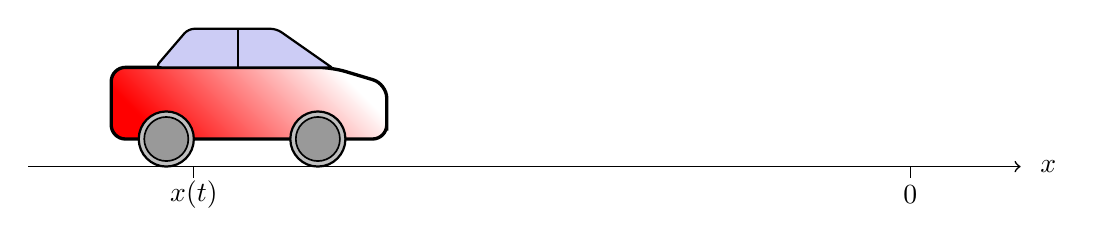
\begin{tikzpicture}[x=-0.7cm,y=0.7cm]
    \shade[top color=red, bottom color=white, shading angle={135}]
        [draw=black,fill=red!20,rounded corners=1.2ex,very thick] (1.5,.5) -- ++(0,1) -- ++(1,0.3) --  ++(3,0) -- ++(1,0) -- ++(0,-1.3) -- (1.5,.5) -- cycle;
    \draw[very thick, rounded corners=0.5ex,fill=black!20!blue!20!white,thick]  (2.5,1.8) -- ++(1,0.7) -- ++(1.6,0) -- ++(0.6,-0.7) -- (2.5,1.8);
    \draw[thick]  (4.2,1.8) -- (4.2,2.5);
    \draw[draw=black,fill=gray!50,thick] (2.75,.5) circle (.5);
    \draw[draw=black,fill=gray!50,thick] (5.5,.5) circle (.5);
    \draw[draw=black,fill=gray!80,semithick] (2.75,.5) circle (.4);
    \draw[draw=black,fill=gray!80,semithick] (5.5,.5) circle (.4);

    \draw[<-,semithick] (-10,0) -- (8,0);
    \draw (-10.5,0) node {$x$};
    \draw (5,0) -- (5,-.2);
    \draw (5,-.5) node {$x(t)$};
    \draw (-8,0) -- (-8,-.2);
    \draw (-8,-.5) node {$0$};
\end{tikzpicture}
\end{center}

Pour cela il envoie un signal $s(t)$.

\begin{questions}
    \questioncours Propagation unidimensionnelle d'une onde progressive. Cas des ondes électromagnétiques dans le vide. Déterminer $s(x,t)$.
    \uplevel{\`A l'instant $t = 0$, l'émetteur envoie un train d'ondes puis un second à
l'instant $t = T$, où $T$ est donc la période d'émission des trains d'ondes. Le signal se réfléchit ensuite sur le véhicule et revient vers le }
    \question Exprimer la période $T'$ perçue par le véhicule.
    \question De même exprimer la période $T''$ perçue par le récepteur du radar et montrer que
    $$f'' = \dfrac{1 + v/c}{1 - v/c}f \stackrel{v \ll c}{\simeq} 1 + 2\dfrac{v}{c}.$$
    \question Le radar envoie un signal sinusoidal de fréquence $f = \SI{24.125}{GHz}$. Interpréter le signal reçu :
\begin{EnvUplevel}
    \centering
    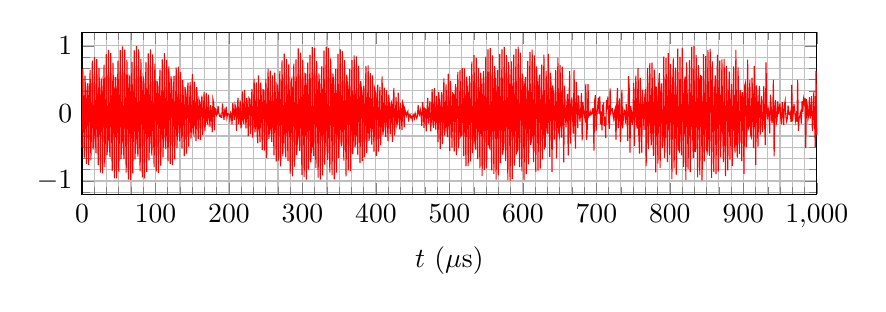
\begin{tikzpicture}
    \begin{axis}[
     clip=false,
     xmin=0,xmax=1000,
     xlabel= $t$ ($\mu$s),
     %axis lines=left,
     %axis x line=middle,
     %axis y line=left,
     width=.9\linewidth,
     height=.3\linewidth,
     ytick={},
     grid=both,
     minor tick num=5,
     ]
      \addplot[domain=0:1000,samples=1000,red]{0.5*sin(deg(x)*1e3)+0.5*sin(deg(x+.3)*(1e3+1.6e-7*24.125*1e3*2*pi))};
      %\addplot[domain=0:1000,samples=200,black,dashed]{cos(deg(x)*1.6e-7*24.125*1e3*pi)};
      %\addplot[domain=0:1000,samples=200,black,dashed]{-cos(deg(x)*1.6e-7*24.125*1e3*pi)};
    \end{axis}
  \end{tikzpicture}
\end{EnvUplevel}
Le véhicule respecte-t-il la limitation en vigueur ?
\uplevel{Pour que le signal soit plus exploitable, on effectue une détection synchrone : le signal reçu $s(t)$ est multiplié par le signal émis $s_0(t)$ et on lui applique un filtre qui coupe les fréquences plus grandes ou égales à $f$.}
    \question Quel est alors ce nouveau signal $g(t)$ ? En quoi ce nouveau signal est plus simple ?
\end{questions}
  

\end{exercise}

\begin{solution}
\begin{questions}
    \question Propagation : $s(x,t) = s(x - ct)$ à droite et $s(x,t) = s(x+ct)$ à gauche.
    \question $T' = \dfrac{1}{1+v/c}T$.
    \question $T'' = (1+v/c)T' = \dfrac{1-v/c}{1+v/c}T$.
    \question 88 km/h
    \question Montage 258
\end{questions}
\end{solution}
% Niveau :      PCSI
% Discipline :  Ondes signaux
% Mots clés :   Propagation des ondes

\begin{exercise}{Sono pourrie}{2}{Sup,Spé}
{Ondes,Propagation des ondes,Doppler}{bermudez}

\noindent\textsfbf{Problème ouvert}

Lors d'un concert de Ariana Grande à Bercy, vous avez le malheur de vous trouver au rang ZC à 150 m de la scène. La salle est approximativement de dimensions $\mathrm{150\,m\times 350\,m \times 30\,m}$. Les haut parleurs émettent la musique de part et d'autre de la scène, qui fait 30 mètres de long.

En quoi cette configuration risque d'altérer votre expérience de spectateur ?

\end{exercise}

\begin{solution}

On superpose deux signaux, modélisés comme sinusoidaux mais légèrement déphasés à cause d'une différence de propagation.

Soit la différence entre les deux haut-parleurs. Soit la différence entre le son direct et le son réfléchi sur le plafond. On peut regarder la différence entre les oreilles aussi.

On pourra étudier le temps d'écho également.
\end{solution}